%%%%%%%%%%%%%%%%%%%%%%%%%%%%%%%%%%%%%%%%%
% Beamer Presentation
% LaTeX Template
% Version 1.0 (10/11/12)
%
% This template has been downloaded from:
% http://www.LaTeXTemplates.com
%
% License:
% CC BY-NC-SA 3.0 (http://creativecommons.org/licenses/by-nc-sa/3.0/)
%
%%%%%%%%%%%%%%%%%%%%%%%%%%%%%%%%%%%%%%%%%

%----------------------------------------------------------------------------------------
%	PACKAGES AND THEMES
%----------------------------------------------------------------------------------------

\documentclass{beamer}

\mode<presentation> {

% The Beamer class comes with a number of default slide themes
% which change the colors and layouts of slides. Below this is a list
% of all the themes, uncomment each in turn to see what they look like.

%\usetheme{default}
%\usetheme{AnnArbor}
%\usetheme{Antibes}
%\usetheme{Bergen}
%\usetheme{Berkeley}
%\usetheme{Berlin}
%\usetheme{Boadilla}
%\usetheme{CambridgeUS}
%\usetheme{Copenhagen}
%\usetheme{Darmstadt}
%\usetheme{Dresden}
%\usetheme{Frankfurt}
%\usetheme{Goettingen}
%\usetheme{Hannover}
%\usetheme{Ilmenau}
%\usetheme{JuanLesPins}
%\usetheme{Luebeck}
\usetheme{Madrid}
%\usetheme{Malmoe}
%\usetheme{Marburg}
%\usetheme{Montpellier}
%\usetheme{PaloAlto}
%\usetheme{Pittsburgh}
%\usetheme{Rochester}
%\usetheme{Singapore}
%\usetheme{Szeged}
%\usetheme{Warsaw}

% As well as themes, the Beamer class has a number of color themes
% for any slide theme. Uncomment each of these in turn to see how it
% changes the colors of your current slide theme.

%\usecolortheme{albatross}
%\usecolortheme{beaver}
%\usecolortheme{beetle}
%\usecolortheme{crane}
%\usecolortheme{dolphin}
%\usecolortheme{dove}
%\usecolortheme{fly}
%\usecolortheme{lily}
%\usecolortheme{orchid}
%\usecolortheme{rose}
%\usecolortheme{seagull}
%\usecolortheme{seahorse}
%\usecolortheme{whale}
%\usecolortheme{wolverine}

%\setbeamertemplate{footline} % To remove the footer line in all slides uncomment this line
%\setbeamertemplate{footline}[page number] % To replace the footer line in all slides with a simple slide count uncomment this line

%\setbeamertemplate{navigation symbols}{} % To remove the navigation symbols from the bottom of all slides uncomment this line
}

\usepackage{graphicx} % Allows including images
\graphicspath{ {./Figures/} }

\usepackage{float}

\usepackage{booktabs} % Allows the use of \toprule, \midrule and \bottomrule in tables


%----------------------------------------------------------------------------------------
%	TITLE PAGE
%----------------------------------------------------------------------------------------

\title[Extreme Learning Machine]{Extreme Learning Machine} % The short title appears at the bottom of every slide, the full title is only on the title page

\author{Dang Vu Lam} % Your name
\institute[USTH] % Your institution as it will appear on the bottom of every slide, may be shorthand to save space
{
University of Science and Technology of Hanoi\\ % Your institution for the title page
\medskip
\textit{lam.dv@live.com} % Your email address
}
\date{\today} % Date, can be changed to a custom date

\begin{document}

\begin{frame}
\titlepage % Print the title page as the first slide
\end{frame}

\begin{frame}
\frametitle{Overview} % Table of contents slide, comment this block out to remove it
\tableofcontents % Throughout your presentation, if you choose to use \section{} and \subsection{} commands, these will automatically be printed on this slide as an overview of your presentation
\end{frame}

%----------------------------------------------------------------------------------------
%	PRESENTATION SLIDES
%----------------------------------------------------------------------------------------

%------------------------------------------------
\section{Extreme Learning Machine}
\begin{frame}
    \frametitle{Extreme Learning Machine}
    \tableofcontents[currentsection]
\end{frame}
%------------------------------------------------
\begin{frame}
    \frametitle{Introduction}
    \begin{itemize}
        \item<1-> ELM is an algorithm designed to increase training speed of Single Layer Feedforward Neural network
        \item<2-> Base on analytical method, ELM avoid major drawbacks posed by Backpropagation \cite{huang_extreme_2016}
    \end{itemize}
\end{frame}
%------------------------------------------------
\begin{frame}
    \frametitle{Mathematical Model}
    As a SLFN, ELM model are extremely simple:
    \begin{equation}
        \hat{Y} = w_o H=W_o F(w_i A + \beta)
    \end{equation}
    \begin{equation}
        Y = \hat{Y} + \varepsilon
    \end{equation}
\end{frame}
%------------------------------------------------
\begin{frame}
    \frametitle{Initialization\cite{huang_extreme_2016}}
    \begin{itemize}[<+->]
        \item Non linear weights initialization\\
        During this stage, input weights matrix $w_i$ are initialized
        \item $w_i$ is assigned randomly in range of $[-1,1]$
        \item<2> Linear weights learning\\
        Output weights matrix can then be learned using analytical method as following:
        \begin{equation}
            w_i = Y * H^\dagger
        \end{equation}
        where $H^\dagger$ is the Moore - Penrose psuedoinverse product of hidden layer output $H$
    \end{itemize}
\end{frame}
%------------------------------------------------
\begin{frame}
    \frametitle{Experiment: Salary Dataset}
    \begin{table}[H]
        \begin{center}
            \caption{Sample from Salary Dataset}
            \begin{tabular}{c c c c c c c }
                Gender & Rank & YOE & Degree & YOR & Salary\\\hline
                male & full & 25 & doctorate & 35 & 36350 \\ 
                male & full & 13 & doctorate & 22 & 35350\\ 
                male & full & 7 & doctorate & 13 & 27959\\ 
                female & full & 8 & doctorate & 24 & 38045\\ 
                female & assistant & 1 & doctorate & 1 & 16686\\ 
                female & assistant & 1 & doctorate & 1 & 15000\\ 
                male & full & 10 & doctorate & 23 & 28200\\ 
                
            \end{tabular}
            \label{tab:sample}
        \end{center}
    \end{table}
\end{frame}
%------------------------------------------------
\begin{frame}
    \frametitle{Experiment: Result}
    \begin{figure}[H]
        \begin{center}
            \includegraphics [width=\textwidth] {result}
        \end{center}
        \caption{Result of ELM experiments on Salary Dataset} 
        \label{fig:plot_result}       
    \end{figure}
\end{frame}

%------------------------------------------------
\section{Particle Swarm Optimization}
\begin{frame}
    \frametitle{Particle Swarm Optimization}
    \tableofcontents[currentsection]
\end{frame}
%------------------------------------------------
\begin{frame}
    \frametitle{Overview}
    \begin{itemize}
        \item<1-> Particle Swarm Optimization is a swarm optimization technique model after the movement of a swarm of animals such as a school of fish or a flock of bird.\cite{eberhart_new_1995}. 
        \item<2> Originally designed to model social behavior, it is later realized to be a powerful tool for optimization problem.
    \end{itemize}
\end{frame}
%------------------------------------------------
\begin{frame}
    \frametitle{Algorithm}
    \begin{equation}
        V_{t+1} = V_t + c1*(global\_best - X_t) + c2*(local\_best - X_t)
    \end{equation}
    \begin{equation}
        X_{t+1} = X_{t} + V_{t+1}
    \end{equation}
\end{frame}
%------------------------------------------------
\begin{frame}
    \frametitle{Result}
    \begin{center}
        For a 100 neurons wide network, a 10 times repeated test yield
    \end{center}
    \begin{equation*}
        \overline{RMSE} = 1209.35099702    
    \end{equation*}
    \begin{equation*}
        \overline{\sigma} = 775.870695031
    \end{equation*}
\end{frame}
%------------------------------------------------
\section{Application of ELM and PSO - ELM}
\begin{frame}
    \frametitle{Application of ELM and PSO - ELM}
    \tableofcontents[currentsection]
\end{frame}
%------------------------------------------------
\begin{frame}
    \frametitle{Deep ELM frameworks}
    \begin{itemize}
        \only<1>{\item Autoencoder - ELM\cite{cao_building_2016}}
        \only<2>{\item Deep ELM - Stacked Autoencoder \cite{cao_building_2016}}
        \only<3>{\item Hierarchical ELM \cite{tang_extreme_2016}}
    \end{itemize}
    \only<1>{
    \begin{figure}[h]
        \begin{center}
            \makebox[\textwidth][c]{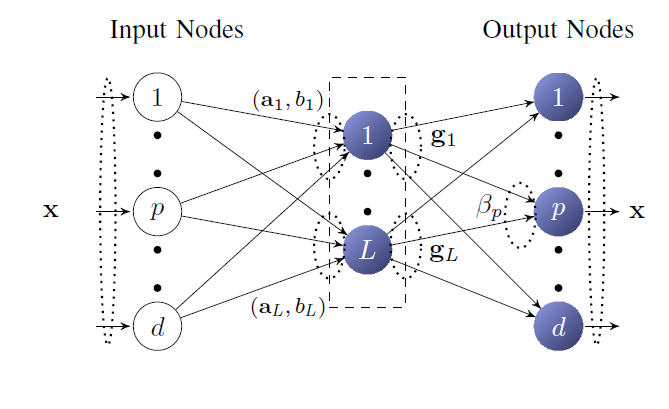
\includegraphics[width=\linewidth]{AE-ELM}}
        \end{center}
    \end{figure}}
    \only<2>{
    \begin{figure}[h]
        \begin{center}
            \makebox[\textwidth][c]{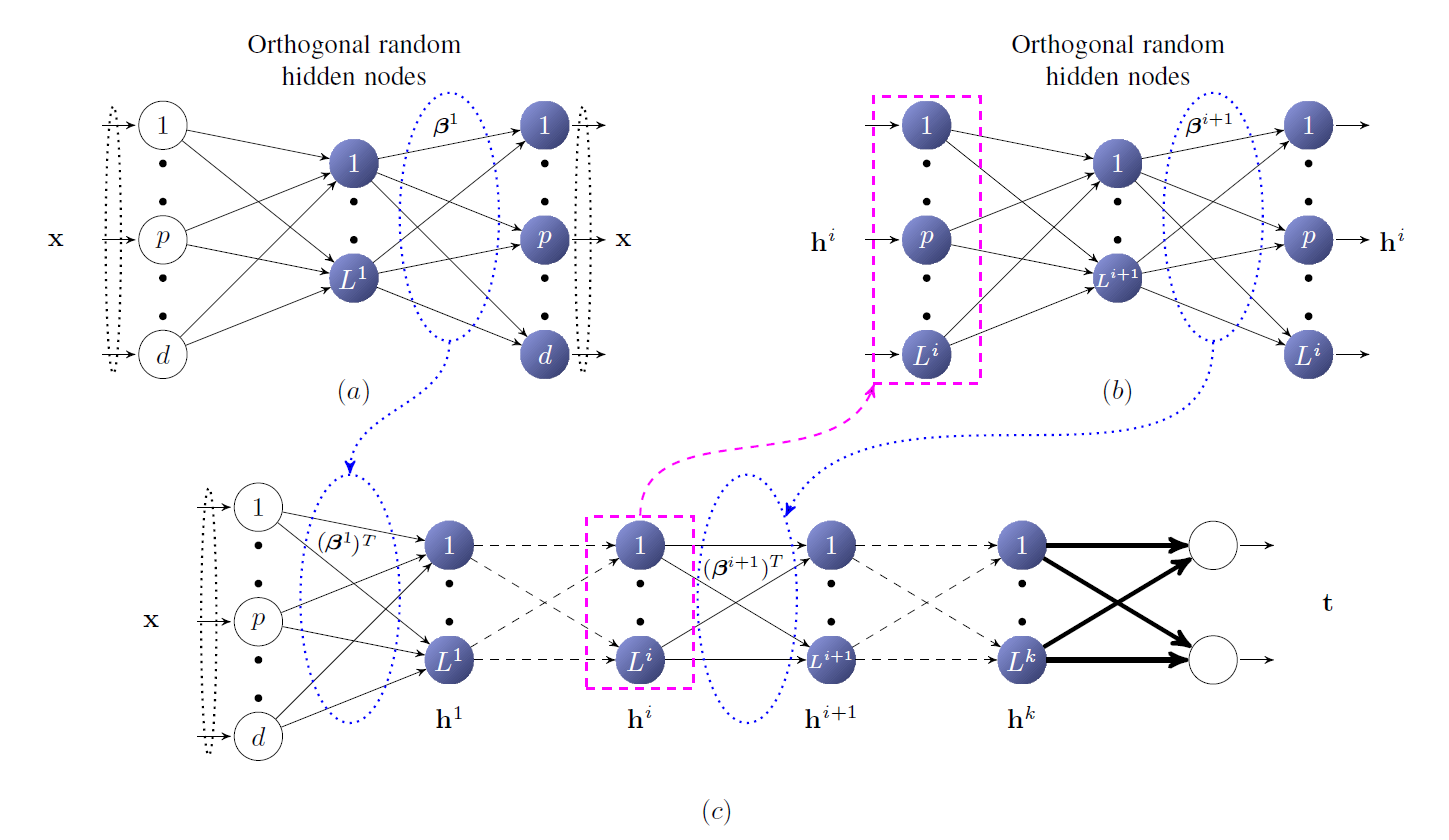
\includegraphics[width=\linewidth ]{Deep-ELM}}
        \end{center}       
    \end{figure}}
    \only<3>{
    \begin{figure}[h] 
        \begin{center}
            \makebox[\textwidth][c]{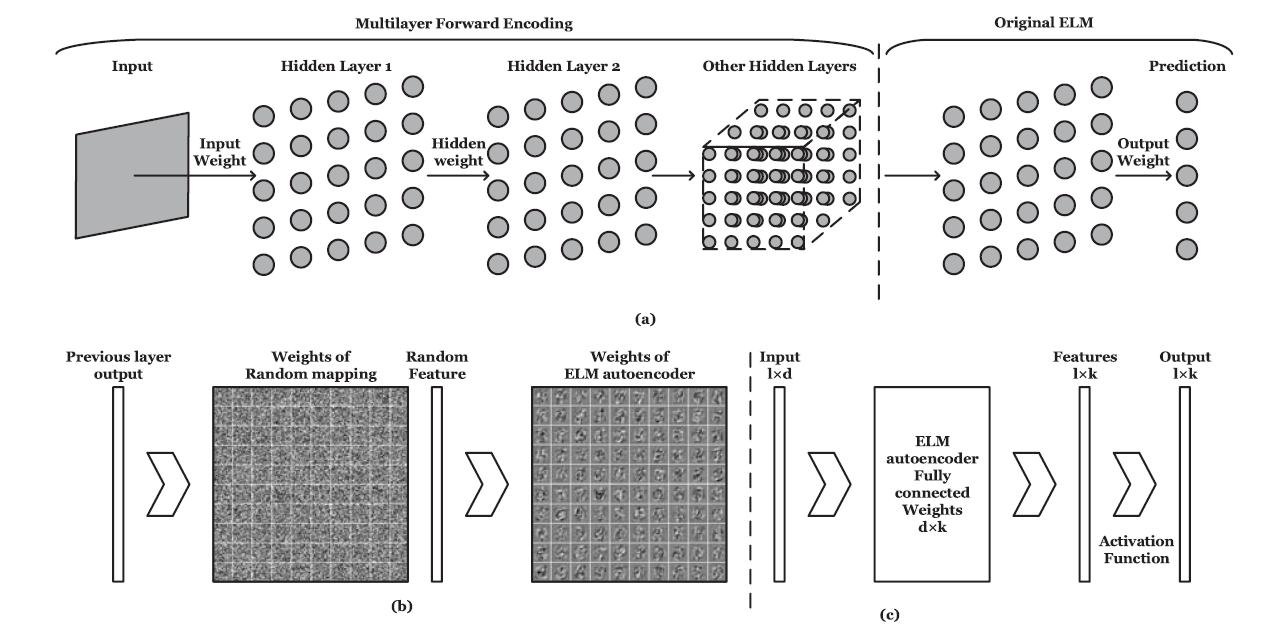
\includegraphics[width=\linewidth ]{H-ELM}}
        \end{center}
    \end{figure}}
\end{frame}
%------------------------------------------------
\begin{frame}
    \frametitle{PSO Optimized Deep ELM}
    \begin{itemize}
        \item <1-> We project that it is possible to tune each layer of the network individually using the method covered in this thesis.
        \item <2-> Such algorithm will have the extra benefit of being able to tune just part of the network rather than the whole network, thanks to the fact that H-ELM is autoencoders stack on top of each other \cite{tang_extreme_2016}.
        \item <3> Since autoencoders transform the input into itself, we also propose a novel method to train each layer separately, independent from each other thus ultilize the capabilities of high performance computing to train all the layer at once, and recombine them according to \cite{cao_building_2016}.
    \end{itemize}
\end{frame}
%------------------------------------------------

\begin{frame}
\frametitle{References}
\bibliographystyle{unsrt}
\bibliography{references,refRnn}
\end{frame}

%------------------------------------------------

\begin{frame}
\Huge{\centerline{Thank you for your attention}}
\end{frame}

%----------------------------------------------------------------------------------------

\end{document} 